\chapter{Data}\label{ch:2}
This chapter introduces the data used in the analysis, motivates the use of non linear models for default prediction and discuss how the data is pre-processed for the models. 

We use the Freddie Mac Single Familiy Loan-Level Dataset for the analysis, which is available to the public at the direction of the regulators \textit{the Federal Housing Finance Agency (FHFA)}, in an attempt to increase data transparency \cite[p. 3]{Freddie_mac_guide}. The data spans from the first quarter of 1999 to the third quarter of 2018 at the time of writing. However, it should be noted that the data is a living dataset, in the sence that it is being updated and additional information could be added or corrected in the future. We downloaded the data at the first February 2020, any changes that may occur after this date will not be taken into consideration. 

The dataset contains approximately 26 million  fully amortising 15, 20 and 20 year fixed-rate mortgages which together have over 2 billion monthly performance updates and together takes up 90GB of space. The data is divided into two csv files one containing the Origination data and another containing the monthly Performance updates. The origination data contains static information given at the origination of the loan while the Performance updates include payment activity for each month. The payment activity variable (cd\_zero\_bal) is used to derive the target variable of the analysis, default of a loan. All the original features of the two datasets are available in Appendix \ref{app:Freddie_mac} Table \vref{tab:FM_origination_features} for the origination features and Table \vref{tab:FM_performance_features}. The features we choose to include in the analysis is listed in Appendix \ref{app:Freddie_mac} Table \vref{tab:included_features}.

The vast amount of data makes the data pre-processing as well as estimation of the models and simply exploring and illustrating the data a challenge using a regular laptop, therefore we choose to use a stratified sample of 50.000 (new) loans per year, having 20 years of data (2018 only 3 quarters) we approximately have 975.000 unique loans with approximately 47.000.000 performance updates. This is still quite a large amount of data, though manageable.  
Our approach for handling the data and building the models is to create a virtual machine on \href{https://cloud.google.com/}{Google Cloud}, which offers \$300 free usage for first time private users. Then we install Ubuntu 18.04, R version 3.6.2 and Rstudio Server, which by typing in the external IP-address and port 8787, we are able to work in Rstudio as we are used to on our laptop, the only difference being that everything is done on Googles servers and not on our own laptop. This is quite nice, as we are able to turn up the processing power and memory when needed, which decreases the estimation time compared to a laptop where these feautures are fixed.

\section{Default Definition}
In the data delivered from Freddie Mac, a variable directly indicating whether or not an obligor have defaulted is not available. One way to define the target variable default interatively through the performance updates and check how many days an obligor is behind on payments which is accordance with current EU regulation \cite[Article 178 1.b]{CRR} which states that >>\textit{..the obligor is past due more than 90 days on any material credit obligation to the institution, the parent undertaking or any of its subsidiaries..}<<. However, since we are analyzing inactive loans and thus have all performance updates in the lifetime of the loan available, we choose define defaulted loans by considering the variable cd\_zero\_bal which holds information on why the balance of the loan became zero. If the zero balance codes are either 03, 06 or 09 we label the loan as defaulted, this method for defining default was also used by \cite{Bhattacharya_2017}.
\begin{flalign} \label{eq:default_definition}
\text{Default} & = \begin{cases} 
            1, \qquad \text{if cd\_zero\_bal = 02, 03, 06 or 09} \\
            0, \qquad \text{otherwise}
            \end{cases}
\end{flalign}

The zero balances codes for defining defaulting loans in plain text is presented below.
\begin{itemize}
    \item[02:] Third Party Sale
    \item[03:] ShortSale or Charge Off
    \item[06:] Repurchase prior to Property Disposition
    \item[09:] REO Disposition
\end{itemize}




\section{Data Cleaning}
In the dataset, there are a small amount of loans with missing data. Missing data can occur from reasons, two potential reason are reporting errors made by the original mortgage vendor or the borrower might have provided incomplete information in the application for the mortgage. 

When considering missing values, we notice that some features are required by the vendor in advance of granting a loan, these features are the FICO (Fair Isaac Corporation) Score, Original Unpaid Balance, Original Interest Rate, if these features are missing we assume it is a reporting error and remove the loan. This removal affects approximately 300.000 loans. 

In this thesis we analyse loans which are no longer active, this means we have the full history of all the loans. The Freddie Mac dataset, does however also include loans which are still active, but these are removed. 
Specifically loans which does not have a final zero balance code in the performance update data are removed. Many of the loans in the dataset are still active, meaning they do not have a zero balance code, thus the dataset is further reduced. 

Table \ref{tab:default_amount} shows the class distribution between default and non-default according to the default definition and the data cleaning process described above. 

\begin{table}[H]
    \centering
    \caption{Class distribution default, non-default}
    \label{tab:default_amount}
    \begin{tabular}{crrr}
    \toprule
         % & \multicolumn{2}{c}{Observations}\\
         % \cmidrule(lr){2-3} \\
         & Default & Non-default & Total\\
         %\cmidrule(lr){2}  \cmidrule(lr){3} \\ 
         Full & & & 984,711 \\
         \# &  22,429 & 657,984 & 680,413\\
         \% &  3.30 & 96.70 & 100\\
        \bottomrule
    \end{tabular}
    \end{table}

There are additional features in the dataset which contain missing values, but not all vendors require this information at loan origination, an example could be the debt-to-income ratio. In these cases we simply impute the missing value using the median. In the case of missing values for categorical variables, we simply add a "U" for unknown. We are aware of the simplification in handling of missing values however, this is not the primary focus of the thesis and thus we will not delve further into this topic. 


\section{Data Exploration}
Working on high dimensional data i.e. a vast amount of observations as well as many variables, exploring the data you are working with is an essential part of developing a good model. Thus we would like to investigate how some key variables from the Freddie Mac dataset are distributed when conditioning on whether the observation defaults or not.  

First we would like to see how the default rate has developed over time. Figure \ref{fig:pw_1}[I] depicts this development. The default rate is calculated by calculating how many loans were active in each year, and then counting the amount of loans defaulting each year. As expected the default rate shows a peak of the default rate in 2008 during the Great Financial Crisis. The default rate had been rising since 2004, and declining in the period after 2009. This shows that the loan performance from 1999 to 2004 were somewhat stable, afterwards from 2004 to 2008 a steep increase happened, and after the crisis 2009-2018 a slow decline occurred. 

% Figure \ref{fig:pw_1}[II] shows the amount of active loans in the period 1999-2018, which peaks in 2009. In this part of the figure, a steep increase of active loans appears from 1999 through 2009, this together with Figure \ref{fig:pw_1}[I] could indicate too many loans were issued to obligors unable to repay the loans. 

\begin{figure}[H]
    \centering
    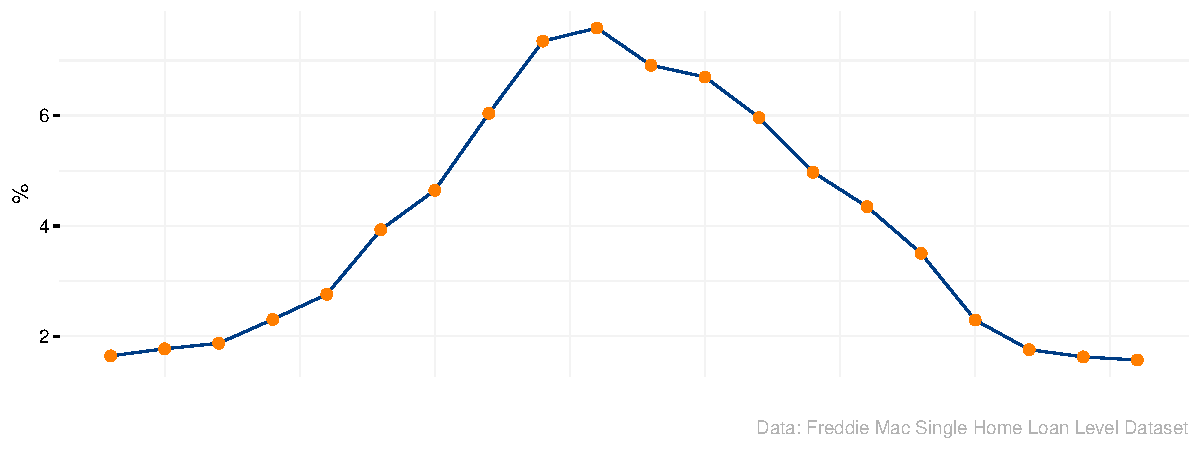
\includegraphics[width = \textwidth]{Figures/pw_1.pdf}
    \caption{Yearly default rate in the Freddie Mac data sample.}
    \label{fig:pw_1}
\end{figure}

Consider Figure \ref{fig:pw_2}[I] where the Default rate is plotted against the Credit Score (FICO). The Figure shows a decreasing relationship between the default rate and the credit score as the credit score increases, indicating a relationship between the FICO score and default rates. This is in line with the results of \cite{Dannis_Pennington_2005},  who for example found credit scores to be an indicator for the quality of the loan. 

Turning to Figure \ref{fig:pw_2}[II] another common and well researched mortgage indicator is depicted against the default rate this is the Loan-To-Value (LTV) ratio. \cite{Ambrose_1998} found higher LTV's to result in higher probability of a mortgage defaulting. Figure \ref{fig:pw_2}[II] is supporting their results, in our data the default rate is increasing as the LTV icreases.  

\begin{figure}[H]
    \centering
    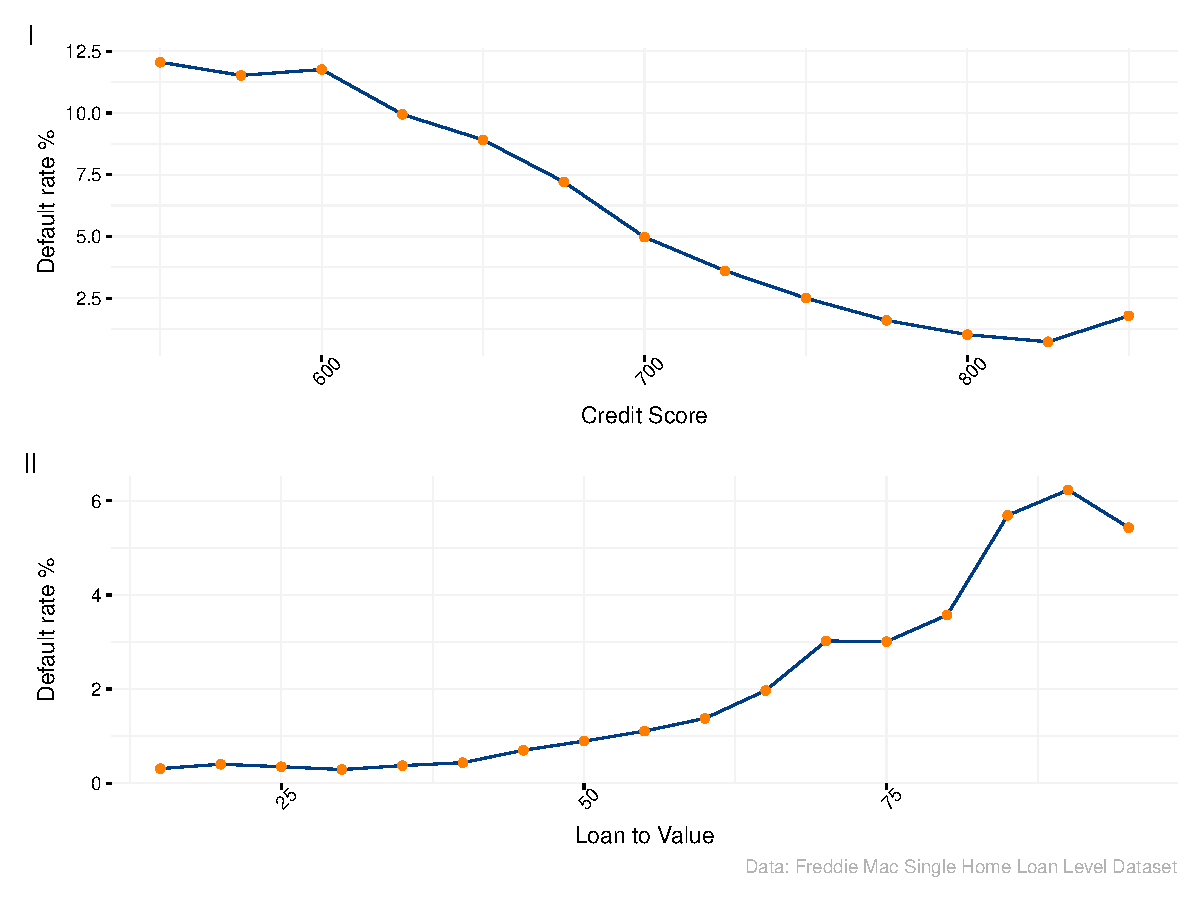
\includegraphics[width = \textwidth]{Figures/pw_2.pdf}
    \caption{Default rate against credit score (FICO) and Loan to Value.}
    \label{fig:pw_2}
\end{figure}

The data also holds the location of the obligors, both by state and by zipcode. In Figure \ref{fig:pw_3}[I] default rates calculated by states are shown, and ordered such that the state with the highest default rates is most to the left. We note that the Florida has the highest default rate in the periode 1999-2018. Another thing to noteice is that California has the most loans of all states, this might not be a surprice, since it is the most populated state in the US. 

Taking the states with the top 5 highest default rates, the development of the default rate for these states are plotted in Figure \ref{fig:pw_3}[II]. Michigan seems to experience increasing default rates earlier than the other 4 states. Figure \ref{fig:pw_3} suggests that the state, could influence defaults. 

\begin{figure}[H]
    \centering
    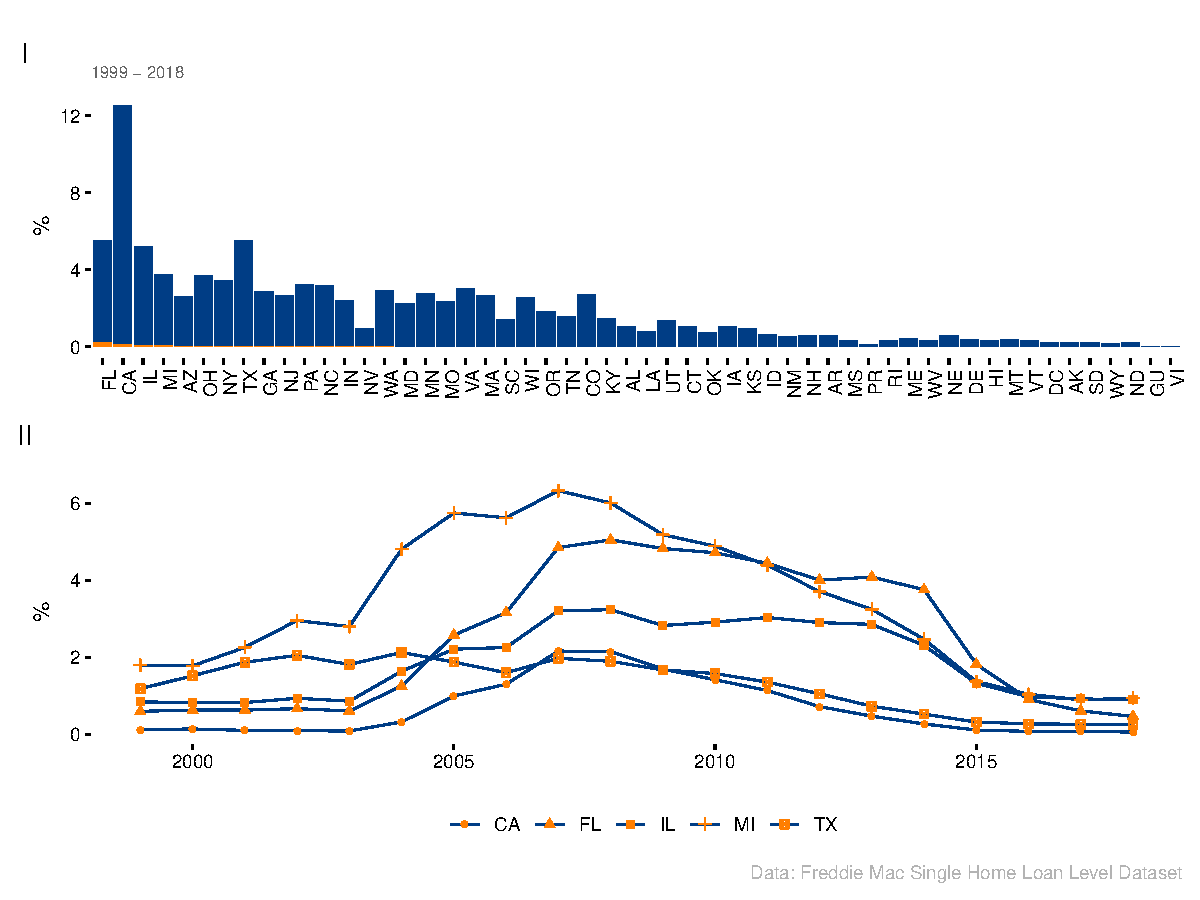
\includegraphics[width = \textwidth]{Figures/pw_3.pdf}
    \caption{Default rates by states.}
    \label{fig:pw_3}
\end{figure}

Figure \ref{fig:pw_5} shows the default- and non-default distributions of 6 selected variables from the origination data. Pane [I] shows the credit score, which we already considered in Figure \ref{fig:pw_2}[I], the takeaway from Figure \ref{fig:pw_5}[I], is that there seem to be some separation of obligors which default and at the same time have a lower credit score compared with obligors who does not default. 

For the Complete Loan to Value shown in Figure \ref{fig:pw_5}[II], the picture is more unclear, but there seem to be a small correlation between higher CLTV ratios and the probability of defaulting. The story is the same for the Loan to Value variable depicted in Figure \ref{fig:pw_5}[III]. 

Regarding the Debt to Income ratio in Figure \ref{fig:pw_5}[VI], higher DTI ratios also have a higher probability of defaulting. The size of the loan is difficult to interpret, the takeaway from Figure Figure \ref{fig:pw_5}[V], must be that the loan amount does not play a role for the probability of defaulting. The last pane Figure \ref{fig:pw_5}[VI] depicts the interest rate default distribution, we note that loans with higher interest rates defaults more often than loans with lower interst rates. This makes sense, since the lower the interest rate the lower the payments (relatively), and since the interest rate reflects the market price of risk, the more risk there is linked with an obligor the more compensation the mortgage institution requires.  


\begin{figure}[H]
    \centering
    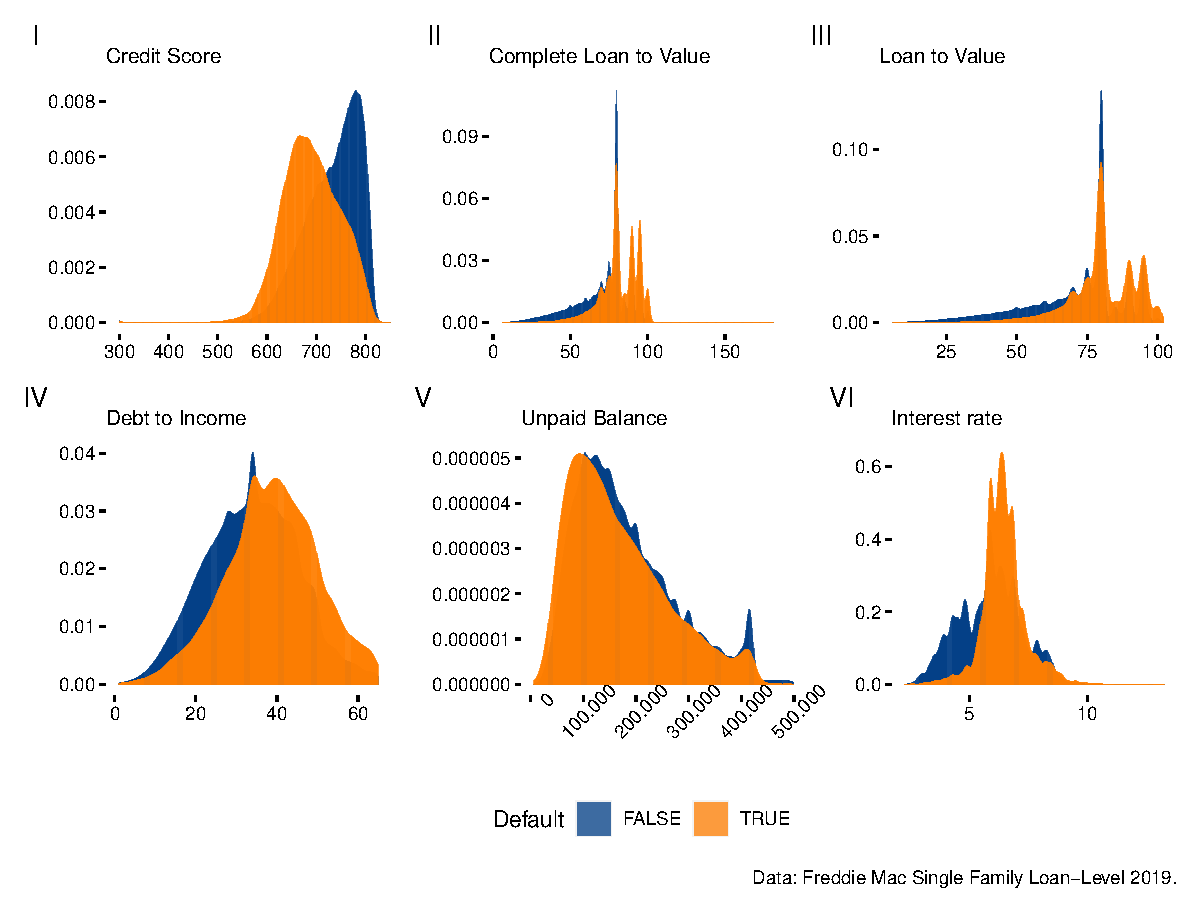
\includegraphics[width = \textwidth]{Figures/pw_5.pdf}
    \caption{Distributions of Credit Score [I], Complete Loan to Value [II], Loan to Value [III], Debt to Income [IV], Unpaid Balance [V] and Interest Rate [VI], divided by the default definition.}
    \label{fig:pw_5}
\end{figure}

The dataset contains many more variables in this part of the thesis we have only shown a selection of the ones available. The distributions for Default and Non-Default, depicted in Figure \ref{fig:pw_5}, are significantly overlapping each other, showing that the data is not linearly separable by these features, and thus motivates the application of non-linear methods, such as Neural Networks, since they are able to model these non-linear relationship and thus out-perform the linear regression models in this classification exercise. 

\textbf{something about creating the features from the performance set...}

use \cite{Chana_2014} and \cite{Sirignano_2018} as references..

Maybe create a figure as 2.4 but of some of the features from the performance vector..

end by refering to a full list of the applied features, is available in the appendix...


\begin{figure}[H]
    \centering
    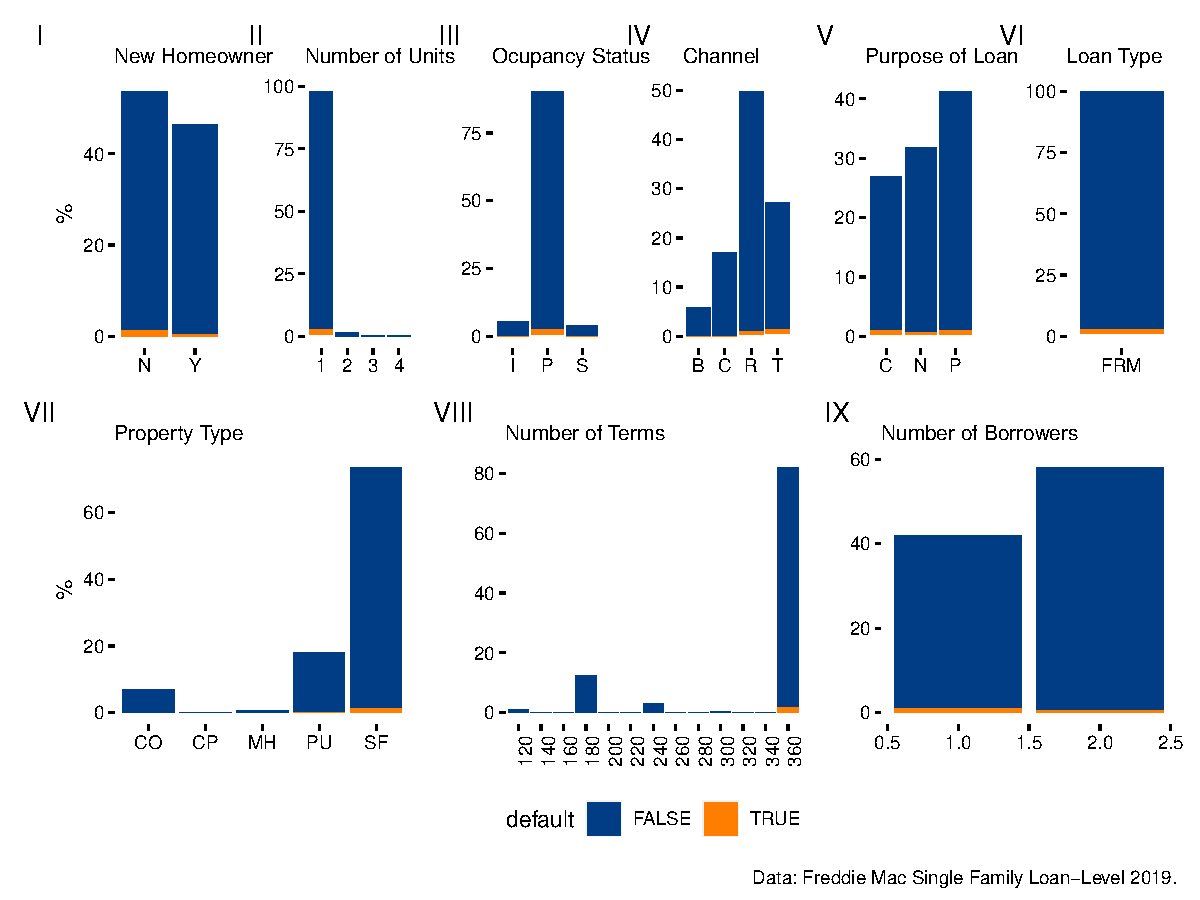
\includegraphics[width = \textwidth]{Figures/pw_4.pdf}
    \caption{Caption}
    \label{fig:my_label}
\end{figure}



\begin{figure}[H]
    \centering
    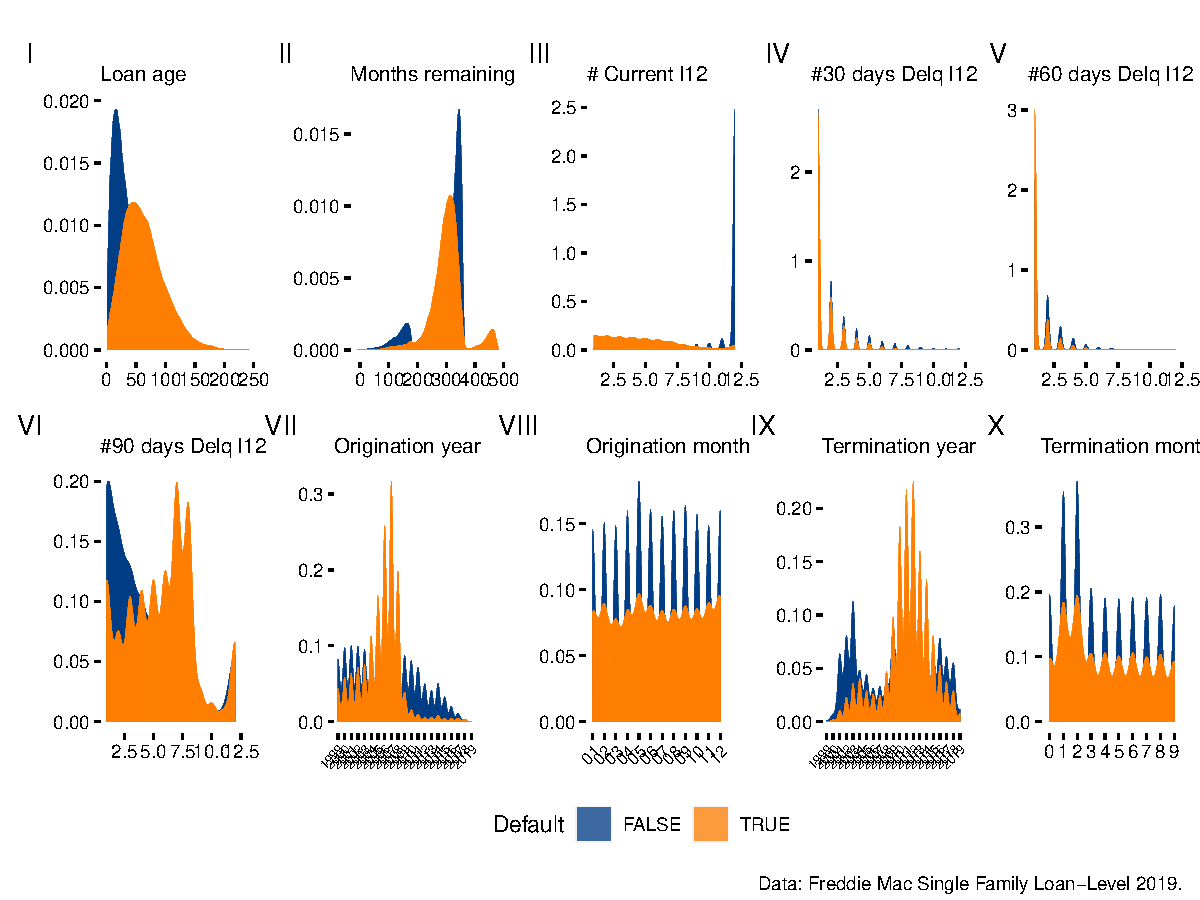
\includegraphics[width = \textwidth]{Figures/pw_7.pdf}
    \label{fig:my_label}
    \caption{Caption}
\end{figure}

        
\section{Data Processing}
    
        \subsection{Implementation}
        
        \subsection{Loading}
        
        \subsection{Manipulation}
        
        \subsection{Model Preparation}
        
    \section{Formal Description}
    
